\documentclass[12pt]{article}
\usepackage{xeCJK}
\usepackage{fontspec}
\usepackage{amsmath}
\usepackage{graphicx}
\usepackage{geometry}
\usepackage{siunitx}
\usepackage{float}
\usepackage{fancyhdr}
\usepackage{circuitikz}
\usepackage{subcaption}
\usepackage{multirow}
\usepackage{cancel}
\setCJKmainfont{Songti SC}
\geometry{a4paper, margin=1in, top=1in}
\setlength{\parindent}{12pt}

\pagestyle{fancy}
\fancyhf{}
\setlength{\headheight}{10pt}
%\fancyhead[L]{\raisebox{-0.5\height}{\includegraphics[width=0.15\textwidth]{pku_logo.png}}}
\fancyhead[R]{\small 普通物理实验报告}
\fancyhead[C]{\small 实验名称：非平衡电桥测量铂电阻温度系数}
\fancyfoot[C]{\thepage}
\renewcommand{\headrulewidth}{0.4pt}
\title{\Large\textbf{非平衡电桥实验报告}}
\author{普通物理实验\\
        [REDACTED]\\
         \\
        姓名：\underline{\hspace{1cm}[REDACTED]\hspace{1cm}} \\
        学号：\underline{\hspace{0.5cm}[REDACTED]\hspace{0.5cm}} \\
        序号：\underline{\hspace{1.3cm}[REDACTED]\hspace{1.3cm}}}
\date{\today}
\begin{document}
\maketitle
\section{摘要}
\quad 本次实验使用非平衡电桥测量了铂电阻的温度系数。实验中，我们首先使用数字万用电表研究铂电阻的封装情况和阻值，然后使用非平衡电桥搭建铂电阻温度计，并进行线性定标。实验中，我们使用三端接法，并使用测量了铂电阻的阻值和温度系数，并进行了误差分析。
\section{测量铂电阻温度系数}
\subsection{条件测量}
\quad 先使用数字万用电表测量铂电阻三端阻值如下：
\begin{equation}
    R_{AB} = 108.49\,\Omega \quad R_{BC} = 108.18\,\Omega \quad R_{AC} = 0.50\,\Omega
\end{equation}
\quad 可以得到，A为铂电阻的单线端，B和C为铂电阻的双线端。
试验采用的非平衡电桥电路图如下：（其中$R_1,R_2$分别使用$10k\Omega$电阻,实测值为$R_1=10.058\,k\Omega , R_2=10.117\,k\Omega$）
\begin{figure}[H]
    \centering
    \begin{circuitikz}[scale=1.5]
        % 电源和电桥上部分
        \draw (0,0) to[short] (0,2);
        \draw (0,2) to[generic, l=$R_1$] (2,2);
        \draw (4,2) to[short] (4,0);
        
        % 电桥下部分
        \draw (0,0) to[generic, l=$R_2$] (2,0);
        \draw (2,0) to[generic, l=$R_0$] (3.6,0);
        
        % 铂电阻三线接法（放在R2位置）
        \draw (2,2) to[generic=*-*, l=$r_1$, resistors/scale=0.4] (2.4,2) to[generic,l=$R_{pt}$] (3.6,2);
        \draw (3.6,0) to[short] (3.6,1.4);
        \draw (3.6,1.4) to[generic=*-*, l=$r_2$, resistors/scale=0.4] (3.6,2);
        \draw (3.6,2) to[generic=*-*, l=$r_3$, resistors/scale=0.4] (4,2);
        % 检流计
        \node[draw,circle,inner sep =3pt] (V) at (2,1) {\footnotesize mV};
        \draw (2,0) to[short] (2,0.75);
        \draw (2,1.25) to[short] (2,2);
        % 电源
        \draw (0,-1) to[short] (0,0);
        \draw (0,-1) to[short] (1.5,-1);
        \draw (1.5,-1) to[battery2, l_=$E$] (2.5,-1);  % 将E的标签改到底下
        \draw (0,-0.5) to[short] (1.75,-0.5);
        \node[draw,circle,inner sep =3pt] (V) at (2,-0.5) {\footnotesize V};
        \draw (2.25,-0.5) to[short] (4,-0.5);
        \draw (2.5,-1) to[short] (4,-1);
        \draw (4,-1) to[short] (4,0);
        
        % 标记端子
        \node[above] at (1.8,2) {A};
        \node[below] at (3.3,1.4) {B};  
        \node[above] at (4.3,2.2) {C};
        
    % 添加虚线矩形封装Rpt
    \draw[dashed] (2,1.5) rectangle (4.0,2.5);
    \node at (3.0,2.8) {铂电阻};
    \end{circuitikz}
    \caption{非平衡电桥测量铂电阻温度系数（引线电阻三端接法）}
    \label{fig:unbalanced_bridge_3wire}
\end{figure}
\subsection{搭建非平衡电桥铂电阻温度计}
\quad 当铂电阻处于冰点时调节$R_0$使得电桥接近平衡，记录此时的温度和$R_0$阻值：(此时电桥输出恰$0mV$)
\[
    T_0=-0.23\,\text{℃}\quad R_0=100.2\,\Omega
\]
\quad 之后，从冰点升高温度直到沸点，大致均匀记录温度计示数和对应的非平衡电桥输出
\begin{table}[H]
    \centering
    \begin{tabular}{|c|c|c|c|c|c|c|c|c|c|}
        \hline
        $T$/℃ & -0.23 & 10.21 & 23.63 & 37.22 & 51.70 & 63.88 & 76.78 & 88.31 & 100.20 \\
        \hline
        $U$/mV & 0.00 & 7.50 & 17.21 & 26.93 & 37.17 & 45.80 & 54.92 & 63.05 & 71.41\\
        \hline
    \end{tabular}
    \caption{非平衡电桥测量铂电阻温度系数的实验数据}
    \label{tab:unbalanced_bridge_data}
\end{table}
\subsubsection{线性定标和性能评估}
\par
\quad 作$U-T$图，得到搭建的非平衡电桥的温度定标图（输出-输入特性）：(样条插值曲线)
\begin{figure}[H]
    \centering
    \begin{subfigure}[b]{0.4\textwidth}
        \centering
        \includegraphics[width=\textwidth]{img/U-T.pdf}
        \caption{非平衡电桥铂电阻温度计的$U-T$输出-输入特性}
        \label{fig:unbalanced_bridge_data}
    \end{subfigure}
    \hfill
    \begin{subfigure}[b]{0.4\textwidth}
        \centering
        \includegraphics[width=\textwidth]{img/U-T-linear.pdf}
        \caption{非平衡电桥铂电阻温度计的$U-T$线性拟合}
        \label{fig:unbalanced_bridge_linear}
    \end{subfigure}
\end{figure}
进一步做线性拟合，得到U关于T的拟合直线如下：（线性拟合直线）
\begin{equation*}
    U = k\cdot T + b \quad k = 0.71082\,mV/\text{℃} \quad b = 0.32383\,mV \quad r=0.999990
\end{equation*}
\quad 根据拟合结果进行分析，可以得到：
\begin{itemize}
    \item 线性度：拟合直线的回归系数$r=0.999990$,可见该铂电阻温度计在$0$\~{}$100\,\text{℃}$范围内具有良好的线性度。
    \item 灵敏度：由于铂电阻在此范围内的良好线性，灵敏度可以用拟合直线斜率表示：$K = \frac{\Delta U}{\Delta T}=0.71082\,mV/\text{℃}$。
    \item 分辨率：数字表的分辨率为$0.01\,mV$，因此温度计的分辨率为$\frac{0.01\,mV}{0.71082\,mV/\text{℃}}\approx0.014\,\text{℃}$,可见该温度计具有较高的分辨率,其灵敏度能满足测量的需求。
\end{itemize}
\subsubsection{铂电阻在$0\,\text{℃}$的阻值测量}
\quad 基于上述线性定标结果，可以得到铂电阻在$0\,\text{℃}$时对应的非平衡电桥输出为：
\begin{equation*}
    U_{0} = k\cdot 0\,\text{℃} + b = 0.32383\,mV
\end{equation*}
\quad 实验中，电源可以看作恒压源，其$E=18.990\,V$，根据非平衡电桥输出原理（如下图\ref{fig:unbalanced_bridge2}），可以得到非平衡电桥输出与$R_{T}$的关系：
\begin{equation*}
    U = E\cdot\frac{R_2\,R_T-R_1\,R_p}{(R_1+R_T)\,(R_2+R_p)}
\end{equation*}
\begin{figure}[H]
    \centering
    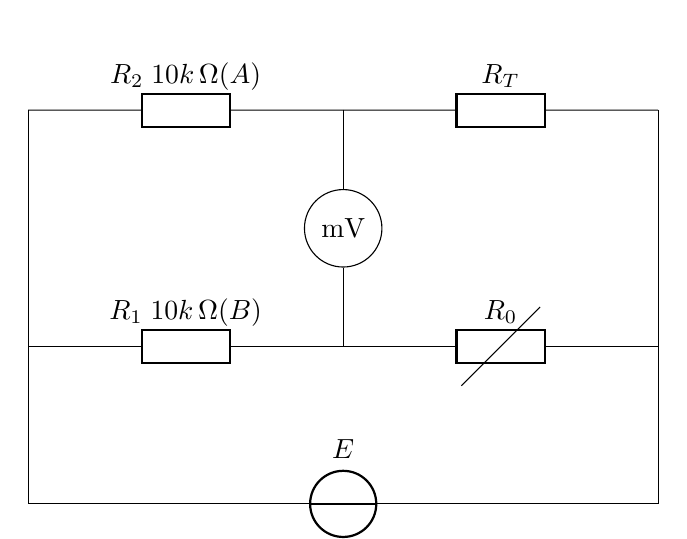
\begin{tikzpicture}
      \draw (0,0) to[generic, l=$R_1 \;10k\,\Omega(B)$] (4,0);
      \draw (4,0) to[generic, l=$R_0$] (8,0);
      \draw (5.5,-0.5) to (6.5,+0.5);
      \draw (0,3) to[generic, l=$R_2 \;10k\,\Omega(A)$] (4,3);
      \draw (4,3) to[generic, l=$R_{T}$] (8,3);
      \draw (4,0) to[short] (4,1);
      \node[draw,circle,inner sep=4pt] at (4,1.5) {mV};
      \draw (4,2) to[short] (4,3);
      \draw (0,3) to[short] (0,-2) to[short] (3,-2) to[V, l=$E$] (5,-2) to [short] (8,-2) to[short] (8,3);
    \end{tikzpicture}
    \caption{非平衡电桥输出原理}
    \label{fig:unbalanced_bridge2}
  \end{figure}
\quad 在电桥平衡位置附近，有:
\begin{equation*}
    R_T \approx R_{T0}+\frac {U}{K'}
\end{equation*}
\quad 其中$R_{T0}$为电桥平衡对应计算得到的的$R_{T}$阻值，$K'=\frac{d\,U}{dR_T}$为$U$对$R_T$的偏导数。计算公式如下：
\begin{equation*}
    R_{T0} = R_0\cdot\frac{R_1}{R_2}=100.2\times\frac{10.058}{10.117}\approx99.62\,\Omega
\end{equation*}
\begin{equation*}
\begin{aligned}
    K'=\frac{d\,U}{dR_T} &= E \cdot \frac{(R_1+R_T)\,R_2-(R_2\,R_T-R_1\,R_p)}{(R_2+R_p)\,(R_1+R_T)^2} \\
    &=E \cdot \frac{R_1}{(R_1+R_{T0})^2} \\
    &\approx 1.85\times10^{-3}\,V/\Omega
\end{aligned}
\end{equation*}
\quad 代入$U_{0}$，可以得到：
\begin{equation*}
    R_{pt0} = R_{T0}+\frac {U_{0}}{K'} = 99.6157\,\Omega + \frac {0.32383\,mV}{1.85098\times10^{-3}V\cdot \Omega^{-1}} \approx 99.79\,\Omega
\end{equation*}
%\begin{figure}[H]
%    \centering
%    \includegraphics[width=0.5\textwidth]{img/unbalanced_bridge.png}
%    \caption{非平衡电桥输出原理}
%    \label{fig:unbalanced_bridge}
%\end{figure}
\quad 从测量结果可以看出，铂电阻阻值精确且在$0\~{} 100\,\text{℃}$范围内有着很好的线性。通过测量输入输出特性内插得到的0℃阻值与标称非常接近，说明拟合结果较为准确。
\subsubsection{铂电阻的温度系数测量}
\quad 工业铂热电阻在$0$\~{} $850\,\text{℃}$范围内具有以下的温度特性
\begin{equation*}
    R_T = R_{pt0}[1+A(T-T_0)+B(T-T_0)^2]
\end{equation*}
其中$R_{pt0}$为$T_0=0\,\text{℃}$时的阻值，$A$为温度系数，$B$为二次项系数。
\par
\vspace{0.4cm}
当铂电阻温度在$0\~{} 100\,\text{}$范围内时，一阶二阶项的大致量级为：
\begin{equation*}
    A(T-T_0)\sim 10^{-1} \quad B(T-T_0)^2\sim 10^{-3}
\end{equation*}
\quad 两者差两个数量级,因此可以忽略二阶项的影响，得到：
\begin{equation*}
    R_T = R_{pt0}[1+A(T-T_0)]
\end{equation*}
\quad 实验中，使用铂电阻温度计测量了$0$\~{} $100\,\text{℃}$范围内的$U-T$特性，线性拟合的斜率为：
\begin{equation*}
    K = \frac{\Delta U}{\Delta T} = \frac{\Delta U}{\Delta R_T} \cdot \frac{\Delta R_T}{\Delta T} = K' \cdot R_{pt0} \cdot A
\end{equation*}
\quad 因此，可以通过输出-输入线性拟合的斜率$K$计算得到温度系数$A$：
\begin{equation}
    A = \frac{K}{K' \cdot R_{pt0}} =\frac {0.71082\,mV/\text{℃}}{1.85098\times10^{-3}V\cdot \Omega^{-1} \cdot 99.7907\,\Omega} \approx 3.8483\times10^{-3}\,\text{℃}^{-1}
\end{equation}
\quad 对比工业铂热电阻的温度系数值$A_0=3.85\times10^{-3}\,\text{℃}^{-1}$，可以发现，实验结果与工业值接近，说明实验结果较为准确。
\subsubsection{铂电阻的温度系数测量不确定度分析}
\quad 根据温度系数的计算公式
\[
    A=\frac{K}{K' \cdot R_{pt0}}
\]
\quad 我们只需要分别计算$K,R_{pt0},K'$的不确定度，然后根据不确定度传递公式计算得到$A$的不确定度。\\
\textbf{1. 温度计灵敏度$K$的不确定度} \\
\par 
$U-T$线性拟合得到的温度计灵敏度的不确定度应该包含：
\begin{itemize}
    \item 线性拟合的误差
    \item 电压测量的允差传递的不确定度
\end{itemize}
\quad 根据线性拟合的误差公式，输出-输入特性曲线的拟合斜率误差为：
\begin{equation*}
    \sigma_{k,fit} = \sqrt{\frac{\frac{1}{r^2}-1}{n-2}} \approx 0.0012 mV/\text{℃}
\end{equation*}
\quad 电压测量的不确定度为：(用测量过程中出现的最大允差（最大测量值）作为保守估计)\\
\par
 实验所用数字万用电表2000$\mu$V档的允差为：
\begin{equation*}
    e=\alpha\%\cdot U_{x} + \beta \% \cdot U_m \quad \alpha=0.05\% \quad \beta \% \cdot U_m=3\text{个字}
\end{equation*}
\quad 于是：
\begin{equation*}
\begin{aligned}
    e_{max,U} &= 0.05\%\cdot 71.41\,mV + 0.03\,mV &\approx 0.066 mV \\
    \sigma_{U} &= \frac{e_{max,U}}{\sqrt{3}} &\approx 0.038 mV 
\end{aligned}
\end{equation*}
\quad 由此带来的不确定度为：
\begin{equation*}
    \sigma_{k,U} = \frac{\sigma_{U}}{\sqrt{\Sigma_{i=1}^{n} (T_i-\overline T)^2}}= \frac{0.03794 mV}{99.32\text{℃}} \sim 10^{-4} mV/\text{℃}
\end{equation*}
\quad 可以发现，拟合误差带来的不确定度远大于电压测量带来的不确定度，因此，温度计灵敏度的不确定度为：
\begin{equation*}
\begin{aligned}
    \sigma_{K} &= \sqrt{\sigma_{k,fit}^2 + \sigma_{kU}^2} \approx \sigma_{k,fit} \approx0.0012\, mV/\text{℃} \\
    \frac {\sigma_{K}}{K} &\approx 1.69\times10^{-3}
\end{aligned}
\end{equation*}
\textbf{2. 铂电阻0℃阻值$R_{pt0}$的不确定度} \\
\par 
接着计算铂电阻0℃阻值$R_{pt0}$的不确定度：(由于$0\text{℃}$和$-0.23\text{℃}$相差不大，修正值较小，因此可以认为$R_{pt0}$的不确定度主要来源于电阻值测量的不确定度：\\
\par
万用电表$20\,k\Omega$档的允差为：$0.2\%\cdot R_x + 0.005\,k\Omega$，因此：
\begin{equation*}
\begin{aligned}
     \frac{\sigma_{R_1}}{R_1} &= \frac{0.2\%\cdot 10.058\,k\Omega + 0.005\,k\Omega}{\sqrt{3}\times 10.058\,k\Omega} &\approx 1.44\times10^{-3} \\
     \frac{\sigma_{R_2}}{R_2} &= \frac{0.2\%\cdot 10.117\,k\Omega + 0.005\,k\Omega}{\sqrt{3}\times 10.117\,k\Omega} &\approx 1.44\times10^{-3} \\
     \frac{\sigma_{R_0}}{R_0} &= \frac{100\times 0.1\%+0.2\times 2\%\,\Omega+0.012\,\Omega}{\sqrt{3}\times 100.2\Omega} &\approx 6.68\times10^{-4}
    \end{aligned}
\end{equation*}
\quad 因此$R_{pt0}$的不确定度为：
\begin{equation*}
\begin{aligned}
    \sigma_{R_{pt0}} &\approx \sigma_{R_{T0}} = R_{T0}\cdot\sqrt{\left(\frac{\sigma_{R_1}}{R_1}\right)^2 + \left(\frac{\sigma_{R_2}}{R_2}\right)^2 + \left(\frac{\sigma_{R_0}}{R_0}\right)^2} \approx 0.21\,\Omega \\
    \frac{\sigma_{R_{pt0}}}{R_{pt0}} &\approx 2.10\times10^{-3}
\end{aligned}
\end{equation*}

\textbf{3. 电桥灵敏度$K'$的不确定度} \\
\par
传递到$K'=\frac{d\,U}{dR_T}=E\cdot \frac{R_1}{(R_1+R_{T0})^2}$的不确定度为：(忽略电源误差)
\begin{equation*}
    \begin{aligned}
        \sigma_{K'} &= \left|\frac{\partial K'}{\partial R_{T0}}\right|\sigma_{R_{T0}} \\
                    &= E\cdot \frac{R_1}{(R_1+R_{T0})^3}\sigma_{R_{T0}}\\
                    &= 18.990\,V\cdot \frac{10.058\,k\Omega}{(10058\,\Omega+99.6157\,\Omega)^3}\cdot 0.2136\,\Omega \\
                    &\approx 3.9\times10^{-8}V\cdot \Omega^{-1} \\
        \frac {\sigma_{K'}}{K'} &= 2.1\times10^{-5}
    \end{aligned}
\end{equation*}
\textbf{综上所述} \\
\par
 温度系数$A=\frac{K}{K' \cdot R_{pt0}}$的不确定度为：
\begin{equation*}
\begin{aligned}
    \frac {\sigma_{A}}{A} &= \sqrt{\left(\frac {\sigma_{K}}{K}\right)^2 + \left(\frac {\sigma_{R_{pt0}}}{R_{pt0}}\right)^2+ \left(\frac {\sigma_{K'}}{K'}\right)^2} \\
        &=\sqrt{\left(1.69\times 10^{-3}\right)^2+\left(2.10 \times 10^{-3} \right)^2 + \left(2.1\times 10^{-5}\right)^2} \\
        &\approx 2.7\times10^{-3}\\
    \sigma_{A} &\approx 0.01\times10^{-3}\,\text{℃}^{-1}
\end{aligned}
\end{equation*}
\quad 因此，铂电阻的温度系数最终测量结果为：
\begin{equation}
    A = (3.85\pm 0.01)\times10^{-3}\,\text{℃}^{-1}
\end{equation}
同上面讨论，结果非常接近于工业铂电阻的参考温度系数。
\section{实验总结与讨论}
\begin{itemize}
    \item 实验中的仪器使用有很多注意要点，比如检流计按下读数，温度计需要预热等。操作过程也较为繁琐，需要耐心细致，比如加热水时温度可能存在\underline{滞后效应}，需要大致判断什么时候停止加热，也需要一直搅拌减小滞后效应。
    \item 实验的数据处理运用了很多处理方法，例如线性拟合后\underline{内插}得到0℃阻值，以及使用不确定度传递公式计算不确定度，线性拟合的斜率不确定度的组成部分等等。
    \item 最终测量结果与标准值较为接近，说明非平衡电桥在测量电阻小变化量时具有很好的灵敏度，同时也体现了铂电阻在$0\~{} 100\,\text{℃}$范围内良好的线性。
    \item 实际测量中的主要误差来源是铂电阻和温度计探头实际温度不相同导致的误差，实验操作中尽可能使得两者空间距离接近，如果进行统一封装可以获得更好的测量结果。
\end{itemize}
\end{document}